% mainfile: ../../../../master.tex
\subsection{RNA Quantification with Qubit\texttrademark~ RNA BR Assay}
% The part of the label after the colon must match the file name. Otherwise,
% conditional compilation based on task labels does NOT work.
\label{task:20180227_cj3}
\tags{lab,rna,qnt}
\authors{cj}
%\files{}
%\persons{}
\sidenote{}

\begin{figure}[H] % position of the figure 
    \centering
    \caption{Illustration for the Qubit\texttrademark~ RNA BR assay}
    \label{fig:20180227_Qubit_RNA_BR}
    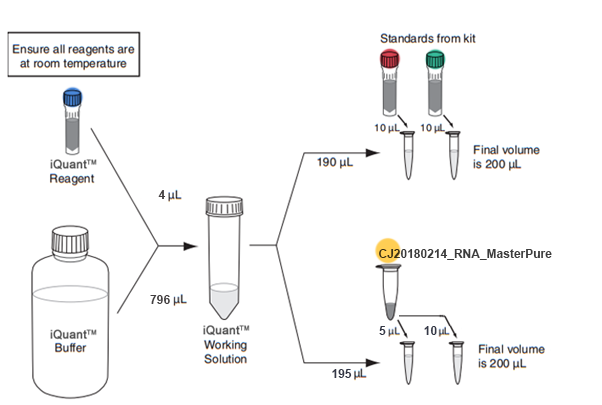
\includegraphics[width=0.8\textwidth]{graphics/schemas/20180215_Qubit_RNA_BR.png}
\end{figure}

\sidenote{I repeated exactly the same as I did on the 20180215.}


\begin{table}[H]
\caption{Total RNA quantities in samples measured with Qubit\texttrademark~ RNA BR Assay Kit}
\label{tab:20180215_rna_qnt}
\centering
\begin{tabular}{l r r r r}
\toprule
Sample ID & \textmu g/mL & $V_f$ (mL) & m (\textmu g) & m (ng) \\ \midrule
\texttt{CJ20180227\_RNA\_AllPrep\_5} & 4.26 & 0.063 & - & - \\
\texttt{CJ20180227\_RNA\_AllPrep\_10} & 3.94 & 0.063 & 0.248 & 248.22 \\
\texttt{CJ20180227\_RNA\_AllPrep\_5} & 4.30 & 0.063 & - & - \\
\texttt{CJ20180227\_RNA\_AllPrep\_10} & 3.95 & 0.063 & - & - \\
\bottomrule
\end{tabular}
\end{table}


My final volume was 80~\uL, but I used 2~\uL for the NanoDrop and 5 and 10~\uL for the Qubit\texttrademark Assay. So my volume is now 63~\uL. Knowing the concentration, I know I actually retrieved at least 315.2 ng of RNA. It's about three time less than what I usually get.
It is surprising that my DNA yield is actually higher than my RNA yield. 

So either the bead beading damages the RNA and not the DNA. Or the maybe the step of drying the RNeasy spin column was very important. 

I must think of other reasons why this happens.